\chapter{FlipIt with virus propagation }
\label{cha:6}
%\documentclass[10pt]{article}\

%%%%%%%%%%%%%%%%%%%%%%%%%%%%%%%%%%%%%%%%%%%%%%%%%%%%%%%%%%
%%%%%			Introduction Chapter 6			%%%%%%
%%%%%												%%%%%%
%%%%%												%%%%%%
%%%%%%%%%%%%%%%%%%%%%%%%%%%%%%%%%%%%%%%%%%%%%%%%%%%%%%%%%%

%\todo{resources vs nodes}
\section{FlipIt vs FlipIt with virus propagation}

This chapter explains how to model a FlipIt game with a virus that propagates and infects the nodes in a network. First, this section explains the difference between FlipIt with and without a virus. 
Then, section \ref{ch:8:GainFlip} derives the formula to calculate the gain for a FlipIt game without a virus. After that section \ref{ch:8:GainVirus} introduces a modification to this formula to achieve an adapted gain formula for a FlipIt game with virus propagation. This allows to derive the benefit formula.\\


\todo{check reff}
In chapter 2 the FlipIt game was explained.  This chapter starts from the specific case of a non-adaptive continuous FlipIt game where both players play a periodic strategy with a random phase. This choice is motivated by the assumption that in the practical situation of most organisations, the defence strategy is to periodically defend the network. This corresponds to a periodic defender strategy. To simplify the analysis in a first time, a periodic attacker strategy is assumed as well. Further research can investigate the effect of relaxing this assumption.\\


A FlipIt game consists of a single resource. To represent the security problem, the game now defines its single resource as a computer network with multiple
nodes. One of the players, the defender, will try to defend his network. The defender
will do this by flipping all the nodes of the network (i.e. the entire resource) in every move he plays. The
attacker, the other player, will try to infect all the nodes in the network. The attacker
will do this by flipping the node in the graph that can infect all the nodes in the
shortest time possible. After dropping a virus on the first node, it takes a while for the virus to infect the entire network. However, since the original FlipIt game works with a single resource that is always flipped entirely, the assumption is made that the attacker is considered to have gained the control over the resource only when all the nodes of the network have been infected, i.e. the entire resource has been flipped. 


\section{Gain formula for a FlipIt game without virus propagation}
\label{ch:8:GainFlip}
In their FlipIt paper [], Marten van Dijk and Ari Juels and Alina Oprea and Ronald L. Rivest, give a definition of the gain of a player \textit{i} . This definition is however not easy to adapt to the situation with virus propagation. Therefore, this section presents an alternative formula that defines a game by quantifying the amount of time each player has control. \\


The following notations will be used throughout the formal definition (see figure \ref{fig:notations} for a graphic representation of some of the notations):

\begin{description}
\item $\delta_{D}$: This is the period of the defender. This denotes the length of the interval between two consecutive moves of the defender. ($\delta_{D} > 0$)
\item $\delta_{A}$: This is the period of the attacker. This denotes the length of the interval between two consecutive moves of the attacker. ($\delta_{A} > 0$)
\item \textit{$T_{D}$}: This denotes the phase of the defender that was chosen randomly and uniformly over the interval [0,$\delta_{D}$].
\item \textit{$T_{A}$}: This denotes the phase of the attacker that was chosen randomly and uniformly over the interval [0,$\delta_{A}$].
\item \textit{Unit of control}: Defined as the period between gaining (full) control and losing control over the resource.  
\item $n_{D}$: The n'th interval of the defender if $\delta_{D} \geq \delta_{A}$ , starting from interval 0.
\item $n_{A}$: The n'th interval of the attacker if $\delta_{A} \geq \delta_{D}$ , starting from interval 0.
\item $\Delta Unit_{D}(n)$ : This is a function that denotes the length of a unit of control of the defender in the n'th interval of the attacker or the defender depending on who is playing faster.
\item $\Delta Unit_{A}(n)$ : This is a function that denotes the length of a unit of control of the attacker in the n'th interval of the attacker or the defender depending on who is playing faster.
\item \textit{lcm(a,b)}: The least common multiple of a and b.
\item \textit{gcd(a,b)}: The greatest common divider of a and b.
\item $G_{i}(t)$: Gain of player \textit{i} at time t. The gain of a player is defined as the total amount of time that a player has owned the resource since the start of the game up to time t. In the context of a FlipIt game with virus propagation, the whole network is seen as one resource. This resource is owned by the attacker if he has control over the entire network.\\
\item \textit{Average Gain}:  $\gamma_{i}(t) = G_{i}(t)/t$ is the average gain rate of player \textit{i} which is defined as the fraction of time that player \textit{i} has control over the resource up to time t.
\item \textit{Benefit}: The average benefit of a player \textit{i} is denoted by $\beta_{i}(t) = \gamma_{i}(t) - k_{i} / \delta_{i}$, which is equal to the fraction of time that the resource has been owned by player \textit{i}, minus the cost rate for moving. For now we consider the cost rate equal to 0.
In the rest of the paper the 'benefit' of the game for player \textit{i} will be used as shorthand for 'average benefit'.

%%------------------------------------------------------------%%
%% Figuur
%%------------------------------------------------------------%%
\end{description}
\begin{figure}[hbtp]
\caption{Graphic representation of some of the notations}
\centering
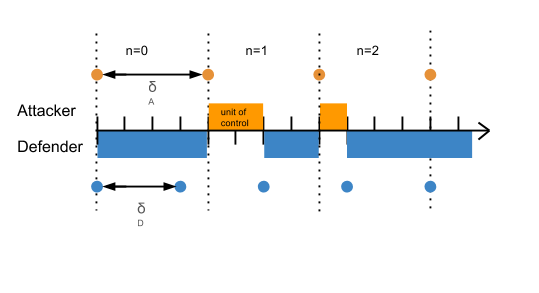
\includegraphics[scale=0.8]{Images/notqties}
\label{fig:notations}
\end{figure}

%To compute the gain of the attacker 
To compute the gain of a player in a periodic game without phases, two cases are considered: case 1 where the defender moves as least as fast as the attacker and case 2 where the attacker plays as least as fast as the defender.  Next, the formula is enriched by introducing the phases.

\subsubsection{Computing the gain for an attacker of a normal FlipIt game}
Consider a game without phases, so in which both players start with a phase $T_{D}$ and phase $T_{A}$ equal to zero. Both players start their first move at $t=0$. As previously stated (in the formal definition of the game and the introduction of different notations used throughout the paper), the defender has control in the beginning of the game at $t=0$. For the remainder of the game, if the two players move at the same time during the game, the moves cancel each other out and no change of state happens. \\

\textbf{Case  1:} \\
$\delta_{A} \geq \delta_{D}$ (The defender moves at least as fast as the attacker.) \\



To compute the gain formula for the attacker,the amount of time that the attacker has control over the game from the start of the game up to time t has to be calculated. This can be done by computing the sum of all the units of control of the attacker up to time t. 


To calculate a single unit of control of the attacker, the time line of the FlipIt game is divided into intervals of size $\delta_{A}$. Every time the attacker moves we have the start of a new interval, with the attacker being in control, unless there is a simultaneous move with the defender. 
Considering that the defender moves at least as fast as the attacker, he or she will at least move one time during the interval of the attacker. Because the attacker only moves at the start of his or her interval we can say that the defender will always end as being in control of the resource. 
\todo{tekening met voorbeeld}. \\

To calculate how long the unit of control of the attacker is in the n'th interval, we only need to know how long the attacker has control over the resource before the defender moves in that interval. The start time of the n'th interval will be a multiple of the period of the attacker. Once the attacker has played, the time he can stay in control until the next move of the defender, depends on the time elapsed since the last time the defender played in the previous interval ( the (n-1)th interval).  

The time the defender plays in an interval is a multiple of its period. Once the defender has played for the last time in the (n-1)'th interval, the remaining time until the attacker will play can be calculated as the remainder of $n\cdot \delta_{A}$ divided by $\delta_{D}$ or $n \cdot \delta_{a}~modulo~ \delta_{D}$. The time the attacker will stay in control is then $\delta_{D}- n \cdot \delta_{A}~ modulo ~ \delta_{D}$, which can also be calculated as $( -n \cdot \delta_{A}) ~modulo~ \delta_{D}$.  

Figure \ref{fig:modulo} illustrates this graphically, for $\delta_{A}= 4$, $\delta_{D}=3$ and the $n=2$ interval. We see that in interval 1, the defender will stay $8 ~modulo~ 3 = 2$ in control, and so, in interval 2, the attacker will stay $1 = 3 - 2 = -(2*4) ~modulo~ 3$ in control.

%%------------------------------------------------------------%%
%% Figuur
%%------------------------------------------------------------%%

\begin{figure}[hbtp]
\caption{Taking the modulo of a negative number}
\centering
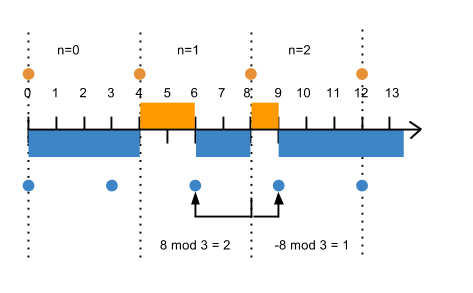
\includegraphics[scale=0.4]{Images/modulotek}
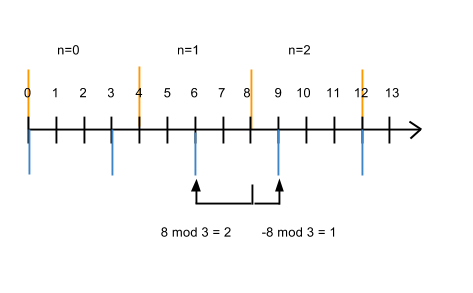
\includegraphics[scale=0.4]{Images/Modulosimpel}
\label{fig:modulo}
\end{figure}


This brings us to the next formula to calculate the length of a unit of control in the n'th interval of the attacker. 

For every positive and non zero real $\delta_{A}$ and $\delta_{D}$ $\in$ \(\mathbb{R}\) and every n $\in$ \(\mathbb{N}\) (including 0 in the set of natural numbers) :
\begin{equation}\label{first}
\Delta Unit_{A}(n_{A}) =  [( - n_{A}  ) \cdot \delta_{A}] mod \delta_{D}
\end{equation}
where $n_{A}$ is the number of the n'th interval of the attacker starting form interval 0 where the length of the unit of control of the attacker is calculated.\\

The length of a unit of control of the defender is the remainder of the interval after the attacker loses control over the resource when the defender plays. This can be defines as follows for the n'th interval of the attacker:
\begin{equation}\label{first}
\Delta Unit_{D}(n_{A}) = \delta_{A} - [( - n_{A}  ) \cdot \delta_{A}] mod \delta_{D}
\end{equation}

An example: Figure \ref{fig:modulo} shows a FlipIt game were the period of the attacker is Pi and the period of the defender is 1. ..\todo{aanvullen}.
On figure \ref{fig:unitofcontrolformula} 

%%------------------------------------------------------------%%
%% Figuur
%%------------------------------------------------------------%%
\begin{figure}[hbtp]
\caption{Example for calculating the control unit in interval 3 for a FlipIt game with period defender = 1 and period attacker = Pi}
\centering
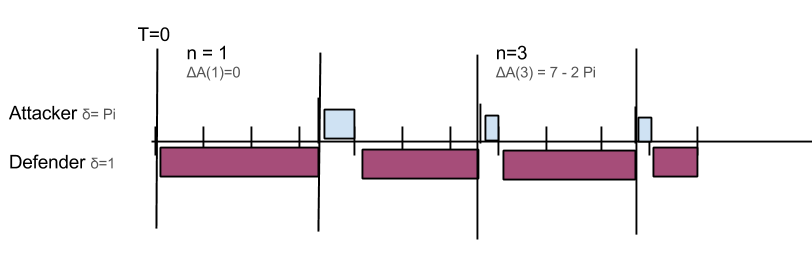
\includegraphics[scale=0.6]{Images/VoorbeeldUnit.png}
\label{fig:unitofcontrolformula}
\end{figure}

The gain formula can be calculated by taking all the units of control of the player up to an amount of p intervals of the attacker. The gain formula for the attacker is stated as follows:

\begin{equation}\label{first}
Gain_{A} = \sum_{i=0}^{p} \lbrace [( - i ) \cdot \delta_{A}] mod \delta_{D}  \rbrace \rbrace 
\end{equation}

where \textit{p} is the number of units of control that have to be summed.  



The gain of the defender is the sum of the units of control of the defender up to the same amount of p intervals of the attacker:
\begin{equation}\label{first}
Gain_{D} = \sum_{i=0}^{p} \lbrace \delta_{A} - [( - i ) \cdot \delta_{A}] mod \delta_{D} \rbrace  \rbrace  
\end{equation}
\begin{equation}\label{first}
Gain_{D} = \sum_{i=0}^{p} \lbrace \delta_{A} \cdot i \rbrace - \sum_{i=0}^{p} \lbrace [( - i ) \cdot \delta_{A}] mod \delta_{D} \rbrace \rbrace  \\
\end{equation}
\begin{equation}\label{first}
Gain_{D} =\delta_{A} \cdot p - \sum_{i=0}^{p} \lbrace [( - i ) \cdot \delta_{A}] mod \delta_{D} \rbrace  \rbrace  \\
\end{equation}

Note: The gain formula is not in function of time t but the amount of p intervals of the attacker. This approach is chosen because it will result in whole units of control. It is possible to make a gain formula using the time, but this will result in a much more complicated function. 


%We know that each interval ends with the control for the defender. This means that we only need to know how long the defender had control during that interval and take the rest. The rest will be the amount of time the attacker has control in that interval. We take the rest by doing the $mod \delta_{0} $

For phases .. \\

\textbf{Case  2:} \\
$\delta_{D} \geq \delta_{A}$ (The attacker moves at least as fast as the defender.) \\

For this case we use the same approach as in case 1 but with a small difference. To compute the unit of control of both players we divide the time line of the FlipIt game into intervals of size $\delta_{D}$.  The defender moves at the start of each interval, the end of the interval is the beginning of the next interval. Considering that the attacker will move at least as fast as the defender, he or she will move at least one time during the interval of the defender. Because the defender only moves in the beginning of each interval, the attacker will end as being in control of the resource.

If the unit of control of the defender need to be calculated, we only need to know how long it takes for the attacker to move in the interval. This can be done in the same way as in case 1 by taking the modulo of the negative of the beginning of the interval. The big difference with case 1 is when the length of the unit of control in the 0'th interval is calculated. Because the defender always has control in the beginning of the game, the first interval is computed in a different way. The unit of control of the defender in the 0'th interval is equal to the length of the period of the attacker, since from that moment the attacker takes control.

For every positive and non zero real $\delta_{A}$ and $\delta_{D}$ $\in$ \(\mathbb{R}\) and every n $\in$ \(\mathbb{N}\) (including 0 in the set of natural numbers) :\\
%\begin{subequations}\label{grp}
%\begin{align}
%a&=b+c\label{second}\\
%d&=e+f+g\label{third}\\
%h&=i+j\label{fourth}
%\end{align}
%\end{subequations} 

\textit{for $n_{A} = 0$}
\begin{equation}\label{first}
\Delta Unit_{D}(n_{D}) = \delta_{A} \\
\end{equation}
\\ 
\textit{for $n_{A} > 0$}
\begin{equation}\label{first}
\Delta Unit_{D}(n_{D}) =  [( - n_{D}  ) \cdot \delta_{D}] mod \delta_{A}\\
\end{equation}
where $n_{D}$ is the number of the n'th interval of the defender starting form interval 0 where the length of the unit of control of the defender is calculated.\\

The length of a unit of control of the attacker is the remainder of the interval after the defender loses control over the resource when the attacker plays. This can be defined as follows for the n'th interval of the defender:
\begin{equation}\label{first}
\Delta Unit_{A}(n_{D}) = \delta_{D} - \Delta Unit_{D}(n_{D})
\end{equation}

The gain formula for $\delta_{D} \geq \delta_{A}$ is calculated in the same manner as case 1:

The gain of the defender is the sum of the units of control of the defender up to the same amount of p intervals of the attacker:
\begin{equation}\label{first}
Gain_{D} =\sum_{i=1}^{p} \lbrace [( - i ) \cdot \delta_{D}] mod \delta_{A} \rbrace   ~~with~~ i=0 ~~ Gain_{D}=\delta_{A}\\ 
\end{equation}

and for the attacker:
\begin{equation}\label{first}
Gain_{A} =\delta_{D} \cdot p - \sum_{i=1}^{p} \lbrace [( - i ) \cdot \delta_{D}] mod \delta_{A} \rbrace   ~~with~~ i=0 ~~ Gain_{A}=\delta_{D} - \delta_{A}\\ 
\end{equation}

\section{Gain and benefit formula for a FlipIt game with virus propagation}
\label{ch:8:GainVirus}
The formulas from the previous section can now be adapted to calculate the gain of both players in a FlipIt game with virus propagation. As mentioned before, the attacker will try to infect all the nodes in the network. He will do this by flipping the node in the graph that can infect all the nodes in the shortest time possible. After dropping a virus on the first node, it takes a while for the virus to infect the entire network. The time that it takes for the virus to infect every node will be denoted as parameter \textit{d}. If we want to measure how long it takes for the virus to infect all the nodes in the network, we have to calculate the shortest path from the
first infected node to the farthest node. This can be measured by a method explained in section [matrix berekeningen]. Assume that an attacker attacks at time t, then only at time t + \textit{d} he gains control over the entire network. If the defender flips the network before the period d has elapsed (so, somewhere between t and t+ \textit{d}), then the attacker will never gain control over the entire network. Using this parameter \textit{d}, a FlipIt game with virus propagation can be modelled.

The previous section defined a formula to calculate each unit of control of the attacker and the defender for two cases. If the virus propagation takes d time before every resource is infected then this \textit{d} has to be subtracted from each unit of control. (see figure 7.4 \ref{fig:virusflip}). It may happen that the unit of control is less than \textit{d}. In that case, the result of the substration will be a negative number, meaning that the defender has flipped all the resources before the attacker could gain control over all the resources. To calculate the gain only the units of control bigger than 0 have to be summed. So the formula becomes: \\

%%------------------------------------------------------------%%
%% Formule
%%------------------------------------------------------------%%

For $\delta_{A} \geq \delta_{D}$ :

\begin{equation}\label{first}
Gain_{A} = \sum_{i=0}^{p} \lbrace [( - i ) \cdot \delta_{A}] mod \delta_{D} - d \rbrace  > 0 \rbrace 
\end{equation}

where \textit{p} is the number of units of control that have to be summed.  

The gain of the defender is equal to the amount of time that the attacker is not in control of the resource. So the formula for the defender becomes:
\begin{equation}\label{first}
Gain_{D} = p \cdot \delta_{A}  -  \sum_{i=0}^{p} \lbrace [( - i ) \cdot \delta_{A}] mod \delta_{D} - d \rbrace  > 0 \rbrace 
\end{equation}

For $\delta_{D} \geq \delta_{A}$ :
\begin{subequations}\label{grp}
\begin{align}
Gain_{A} =\delta_{D} \cdot p - \sum_{i=1}^{p} \lbrace [( - i ) \cdot \delta_{D}] mod \delta_{A} -d \rbrace > 0 \rbrace \\
with~~ i=0 ~~ Gain_{A}=\delta_{D} -( \delta_{A} - d) > 0\\ 
\end{align}
\end{subequations}

and for the defender:
\begin{subequations}\label{grp}
\begin{align}
Gain_{D} =\sum_{i=1}^{p} \lbrace [( - i ) \cdot \delta_{D}] mod \delta_{A} - d \rbrace > 0  \rbrace \\
with~~ i=0 ~~ Gain_{D}=\delta_{A} - d > 0\\ 
\end{align}
\end{subequations}



%%------------------------------------------------------------%%
%% Figuur
%%------------------------------------------------------------%%
\begin{figure}[hbtp]
\caption{Difference in a FlipIt game between delay caused by a virus and a phase bigger than zero for the Attacker}
\centering
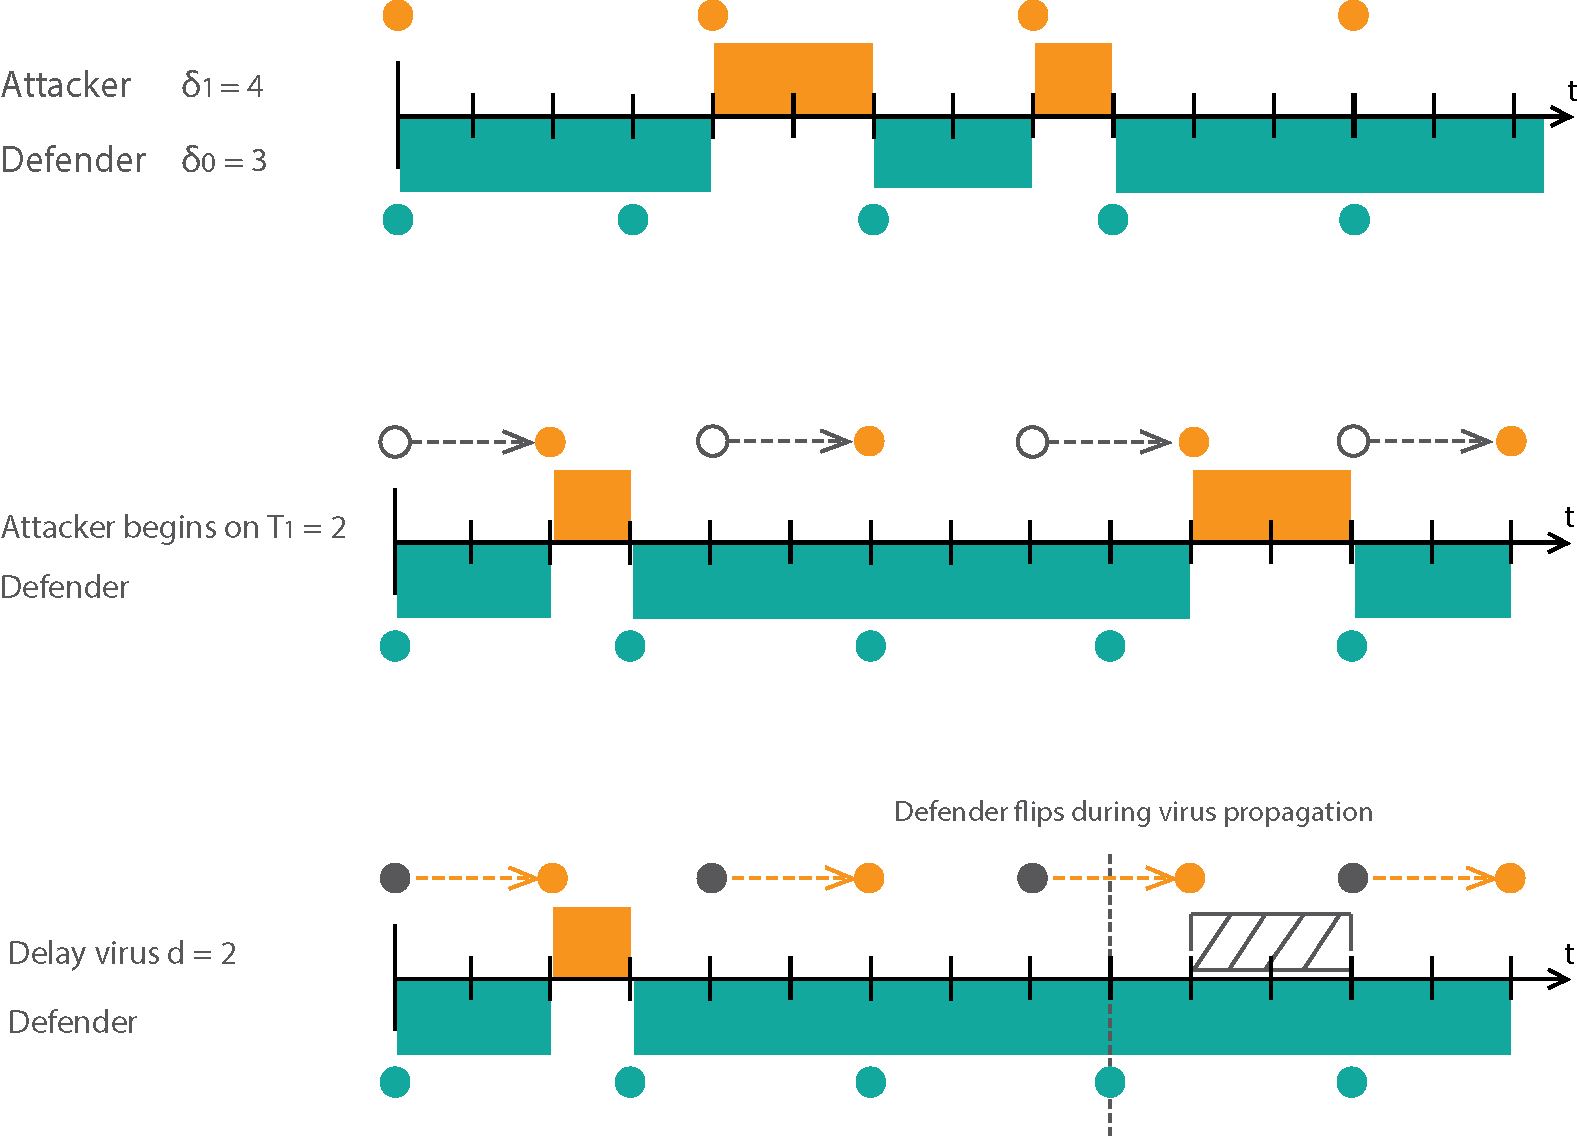
\includegraphics[scale=1]{Images/Flipvirus}
\label{fig:virusflip}
\end{figure}


\subsubsection{Computing the benefit of a FLipIt game with virus propagation}

Calculating the benefit of both players, requires calculating the average gain rate of both players. To compute the benefit the value of parameter \textit{p} needs to be determined. Two cases can be considered: one case where $\delta_{D}$ and $\delta_{A}$ $\in$ \(\mathbb{Q}\) and the other one where $\delta_{D}$ and $\delta_{A}$ $\in$ \(\mathbb{I}.\) In both cases we first calculate the benefit of the attacker in case that the defender moves at least as fast as the attacker. The benefit of the defender will be BenD = 1 - BenA. The benefit of both players for the case where the defender moves as least as fast as the defender is done in a similar way.  \\

\textbf{Rational numbers (\(\mathbb{Q}\)):} When $\delta_{D}$ and $\delta_{A}$ are rational numbers, after a number of intervals (namely their least common multiple), the same pattern of intervals will be repeated over and over again. Why? A rational number is a number that can be expressed as the fraction p/q with p and q $\in$ \(\mathbb{Z}\) (integers), with the denominator q not equal to zero, it is possible to find the \textit{lcm} of $\delta_{D}$ and $\delta_{A}$. The \textit{lcm} is defined for all rational numbers as: $lcm(\dfrac{a}{b},\dfrac{c}{d})= \dfrac{a \cdot c}{gcd(b,d)} with  $ [\todo{referentie}]. When \textit{t} is equal to the \textit{lcm} of $\delta_{D}$ and $\delta_{A}$, both players will move again at the same time and this can be mapped to the beginning of the game. Because we stated that at the end of the interval of the attacker, the defender is in control and because if two players move at the same time the moves cancel each other out, we can map this to the beginning of the game. Since the game goes on infinitely, to calculate the average gain of the attacker, it is sufficient to calculate the average gain of the attacker only during a period of time equal to the \textit{lcm} of $\delta_{D}$ and $\delta_{A}$. Since \textit{lcm} is a multiple of $\delta_{D}$ and $\delta_{A}$, there is a number \textit{p} so that \textit{lcm} $=$p $\cdot \delta_{A}$, meaning that the attacker will have played \textit{p} times. \textit{p} can be defined as follows:


%%------------------------------------------------------------%%
%% Formule
%%------------------------------------------------------------%%
\begin{equation}\label{first}
p = \dfrac{lcm(\delta_{D},\delta_{A})}{\delta_{A} } 
\end{equation}


This results in the following formula for the benefit of the attacker with a cost rate equal to zero:

%%------------------------------------------------------------%%
%% Formule
%%------------------------------------------------------------%%
\begin{equation}\label{first}
\beta_{A} = \dfrac{\sum_{i=0}^{p} \lbrace [[(  - i ) \cdot \delta_{A}] mod \delta_{D} - d] > 0 \rbrace }{lcm(\delta_{D},\delta_{A})} 
\end{equation}

As stated before [], the benefit of the attacker and the benefit of the defender add up to 1 ($\beta_{A} + \beta_{B} = 1$). The benefit of the defender can be writen as follows:
\begin{equation}\label{first}
\beta_{D} = 1 - \beta_{A}
\end{equation}

\textbf{Irrational numbers (\(\mathbb{I}\)):} If $\delta_{0}$ and/or $\delta_{1}$ $\in$ \(\mathbb{I}\):
An irrational number $ i \neq \dfrac{a}{b}$ with $b \in$ \(\mathbb{Z}\) , a $\in$ \(\mathbb{N}\).

Two cases can be distinguished.
(A) $\dfrac{\delta_{D}}{ \delta_{A}}$ is a rational number a/b with a <= b. In that case, after b intervals, the pattern will repeat itself.

(B)If either $\delta_{D}$ and $\delta_{A}$ cannot be written as a fraction, and they are no multiple of each other, the least common multiplier cannot be calculated. Moreover, there will be no repeating pattern. If both players move at one point in the game at the same moment, this point of time has to be a multiple of the period of the attacker and a multiple of the period of the defender. But because there is no least common multiple, no such point of time exists during the game. If both players never play at the same moment, it is not possible to have a repeated pattern because no mapping to the beginning of the game can occur. Additionly two unit of controls with the same length cannot exist. This would mean that the game has a repeated pattern, which is not possible.  \\
The game will go on forever, if no repeating pattern occurs and it would keep on generating units of control with different lengths. This implies that if the game goes on forever, every length between 0 and the smallest interval (which is $\delta_{D}$ ) will be generated.
%If their is no common multiplier the attacker and the defender won't move at one point on the same time, meaning that this does not result in a cycle. If we would have a cycle that means that there exists a number \textit{x} that can be divided by $\delta_{D}$ and $\delta_{A}$. At $t=x$ both of the players will move at the same time, which is not possible because then their would be a cycle. Since their is no cycle it also means that no unit of control will be repeated two times. Every unit of control will have a distinct length. If it does that means that their is repetition, meaning again that their is a cycle. \todo{nog verder uitleggen} We can conclude that if we have no cycle and no number will be repeated twice, that it will enumerate every number between 0 and the biggest interval (which is $\delta_{D}$)
To calculate the benefit we want to summarize the unit of controls up to a number of interval \textit{p}. Considering that the game goes on forever without repetition we cannot rely on the fact that the benefit can also be calculated only during the repetition. Calculating the benefit of a game without repetition would imply that all the unit of control to infinite have to be calculated. This implicates that all the numbers between 0 and   $\delta_{D}$ have to be summed but this is impossible. 
\textit{The reals are uncountable; that is: while both the set of all natural numbers and the set of all real numbers are infinite sets, there can be no one-to-one function from the real numbers to the natural numbers} [WikiPedia: real numbers] If they are uncountable that means that we cannot calculate the sum of all the numbers between 0 and the biggest interval. This is proved by the Cantor diagonalisation argument. Uncountable does not mean that we cannot order it. The Field of the real numbers is ordered. \\

\todo{nog mooie tekst schrijven in engels: hier essentie}
We kunnen de benefit wel benaderen door een zo groot mogelijke som te nemen van de unit of controls. Uit deze benadering is af te leiden waar de verhouding naartoe zou gaan als de limiet zou genomen worden. -> laten zien met een voorbeeld van Pi en 1. 


%What we can do is take the limit, count as many control units of time of the attacker and divide it by the greatest amount of time. We can see that this eventually will result to the solution given by the writers of FlipIt. [r/2]. Example delta1 Pi and delta0 1. Grafiek voor maken.

%\subsection{Random phase}
%For now we assumed that the first move of both players started at phase $t=0$. In the FlipIt game the first move is chosen uniformly over the interval [0,$\delta$]. We will call this first move the phase move and denote it by $T_{1}$ for the attacker and $T_{0}$ for the defender.
%We will have to integrate these two phases into the formula.  
%\begin{equation}      
%\boxed{\eta \leq C(\delta(\eta) +\Lambda_M(0,\delta))}
%\end{equation}
%
%\begin{equation}\label{first}
%a=b+c
%\end{equation}
%
%\begin{subequations}\label{grp}
%\begin{align}
%a&=b+c\label{second}\\
%d&=e+f+g\label{third}\\
%h&=i+j\label{fourth}
%\end{align}
%\end{subequations}



%%% Local Variables: 
%%% mode: latex
%%% TeX-master: "thesis"
%%% End: 


